\chapter{\ifproject%
\ifenglish Experimentation and Results\else การทดลองและผลลัพธ์\fi
\else%
\ifenglish System Evaluation\else การประเมินระบบ\fi
\fi}


\section{Classification model}
\par ผลลัพธ์ จากการ train \& validation ด้วย 3546 sample เป็นจำนวน 200 Epoch

ตัวอย่าง ผลการทดลองของการ validation ด้วย 3546 sample
\begin{figure}[h]
  \begin{center}
  
  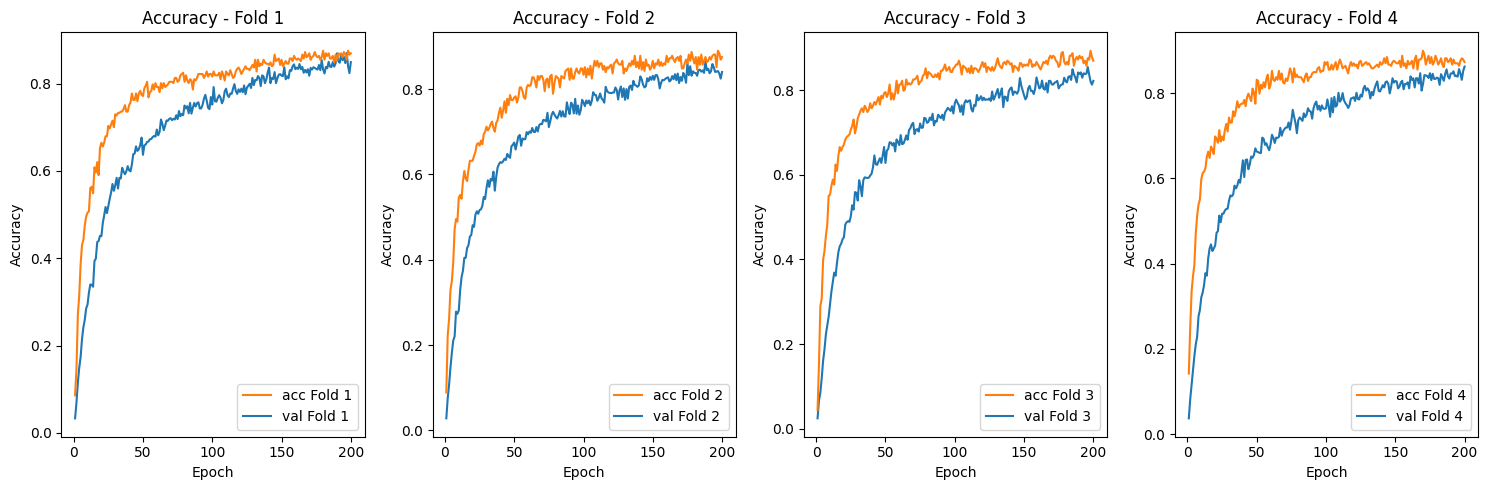
\includegraphics[scale=0.4]{pic/model/train_fold.png}
  \end{center}
  
  \caption[Train fold]{Train fold}
  \label{fig:Train fold}
  \end{figure}

  % โดยเมื่อนำ evaluate มาหา cross_entropy 0.23343226313591003, 0.944695234298706 accuracy

  และทำการเลือก model ที่มีค่า Validation Score สูงสุดจากใน 4 model  
  เพื่อนำไปทำการ Blind Test 
  โดยได้นำ model ใน  Fold 4   มาทำการ
  Evaluate (Blind Test)
  \begin{align}
    \text{cross\_entropy} &= 1.175 \\
    \text{accuracy} &= 0.72
  \end{align}
 
Blind Test

  \begin{figure}[h]
    \begin{center}
    
    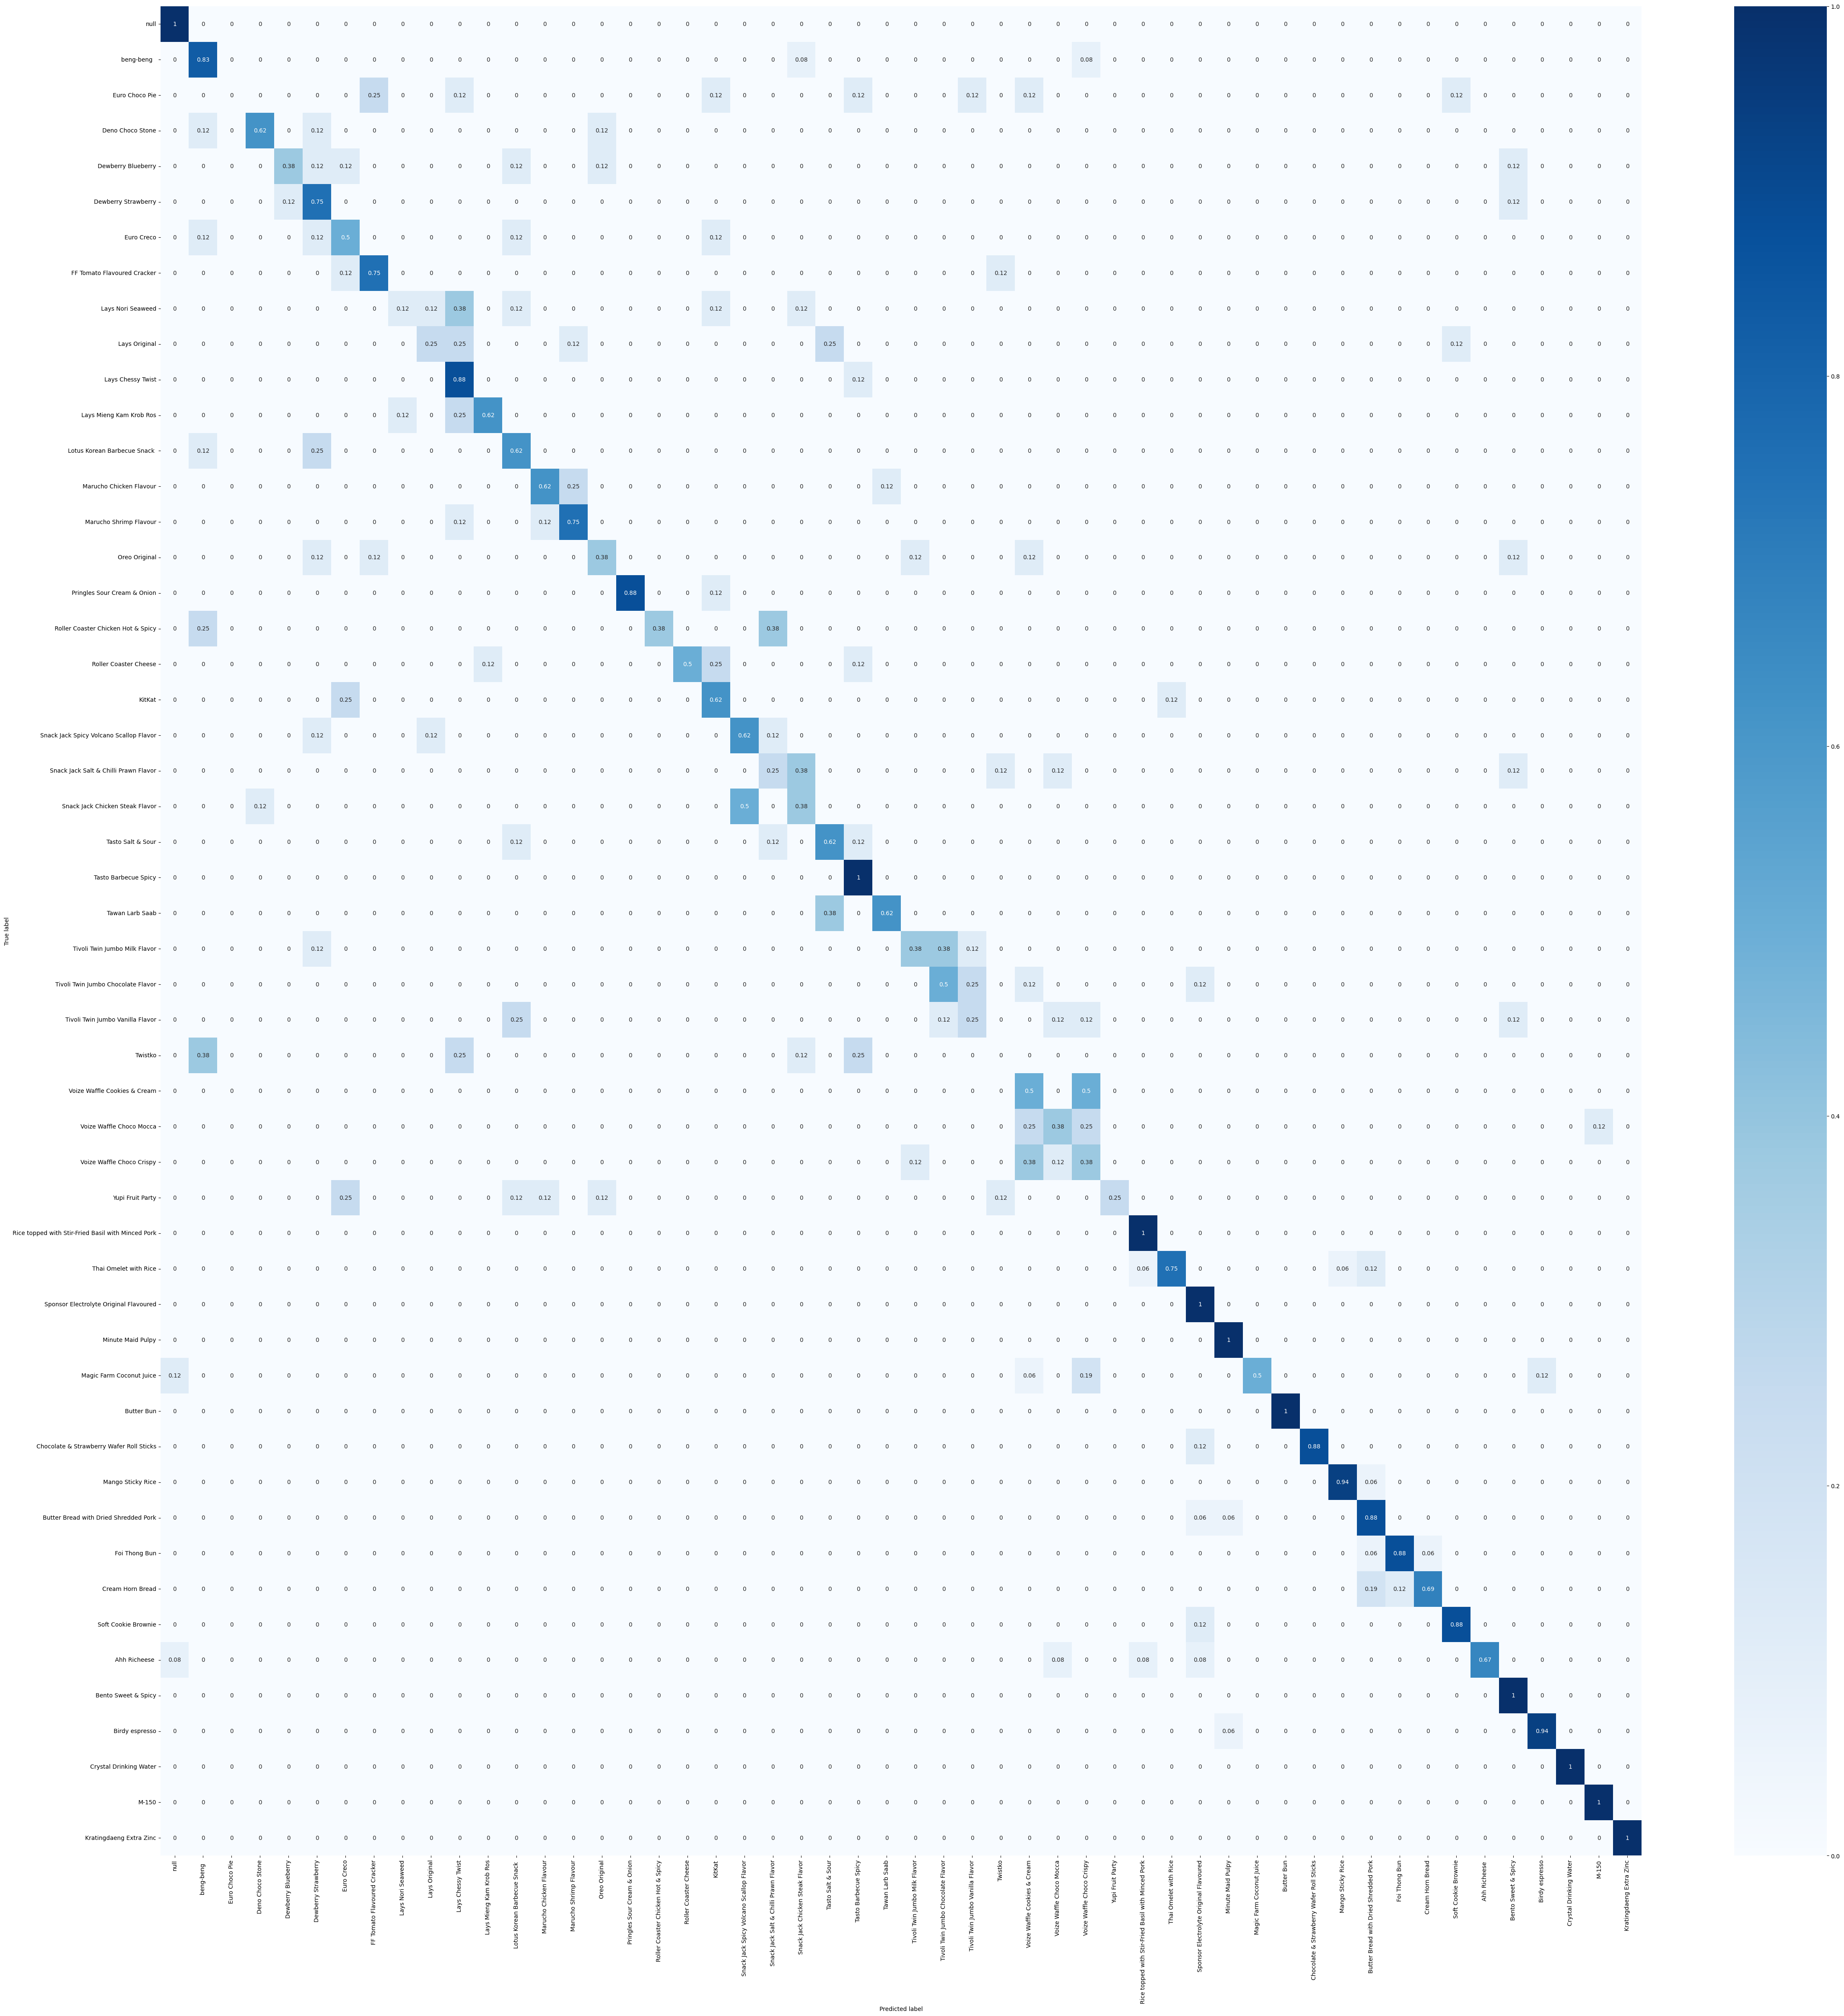
\includegraphics[scale=0.1]{pic/model/blind_pic_4_ccm.png}
    \end{center}
    
    \caption[Confusion matrix]{Confusion matrix}
    \label{fig:Confusion matrix}
    \end{figure}




\newpage
\section{Application UX/UI}

% \begin{figure}[h]
%     \begin{center}
   
%     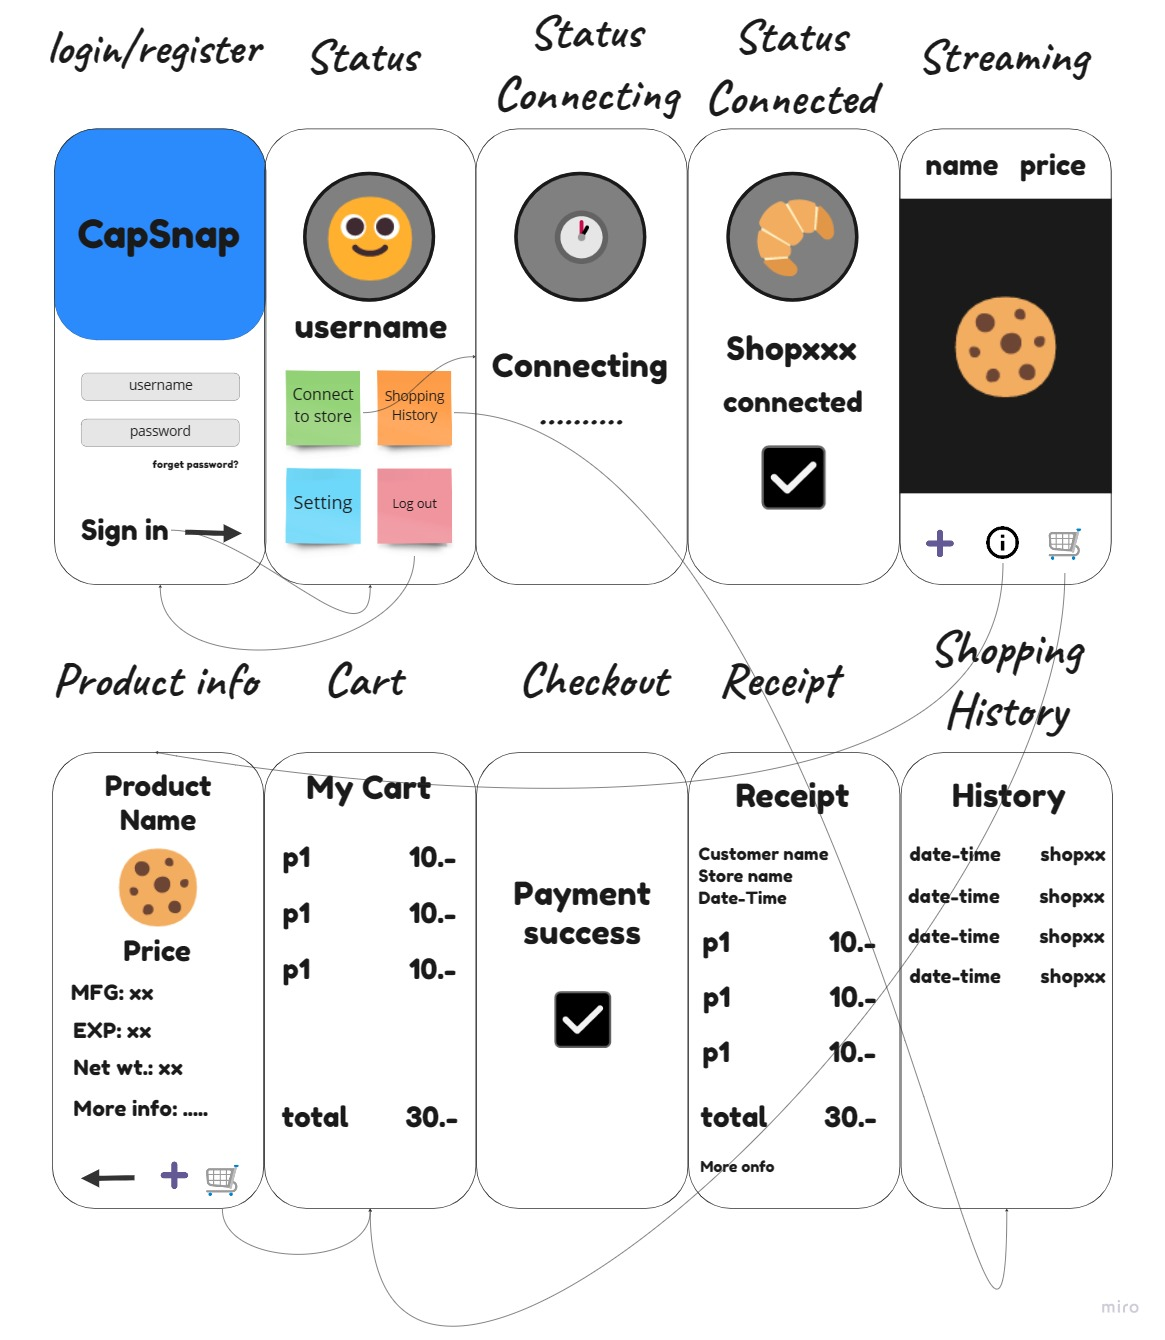
\includegraphics[scale=0.25]{pic/ui/mobileui.jpg}
%     \end{center}
    
%     \caption[Application wire frame]{Application wire frame}
%     \label{fig:Application wire frame}
%     \end{figure} 

ในส่วนของการออกแบบส่วนสื่อประสานกับผู้ใช้ (GUI) ของแอพลิเคชันมือถือนั้น ได้กำหนดให้มีหน้าการใช้งานหลักทั้งหมด 7 หน้า ได้แก่
 
    \begin{enumerate}
        \item Login page: หน้าการเข้าสู่ระบบ 
        \item Register page: หน้าลงทะเบียนเข้าใช้งาน
        \item Home page: หน้าแสดงชื่อผู้ใช้ และเมนูของฟังก์ชันต่าง ๆ
        \item Streaming page: หน้าฟังก์ชันการสตรีมมิ่งรูปภาพสินค้าผ่านกล้องมือถือแบบเรียลไทม์ ซึ่งจะแสดงชื่อ และราคาของสินค้า ซึ่งมีปุ่มการทำงานดังนี้ ปุ่มกดดูรายละเอียดสินค้า ,  ปุ่มเพิ่มสินค้าลงตะกร้า , ปุ่มกดดูสินค้าในตะกร้า
        \item Product Stock page: หน้าแสดงรายละเอียดของสินค้า
        \item My cart page: หน้าแสดง และจัดการเพิ่ม-ลบสินค้าในตะกร้า
        \item History page: หน้าแสดงประวัติการซื้อสินค้า
    \end{enumerate}
 

  

    \begin{figure}
        \begin{center}
            \begin{tabular}{c@{\hspace{3cm}}c}
            
            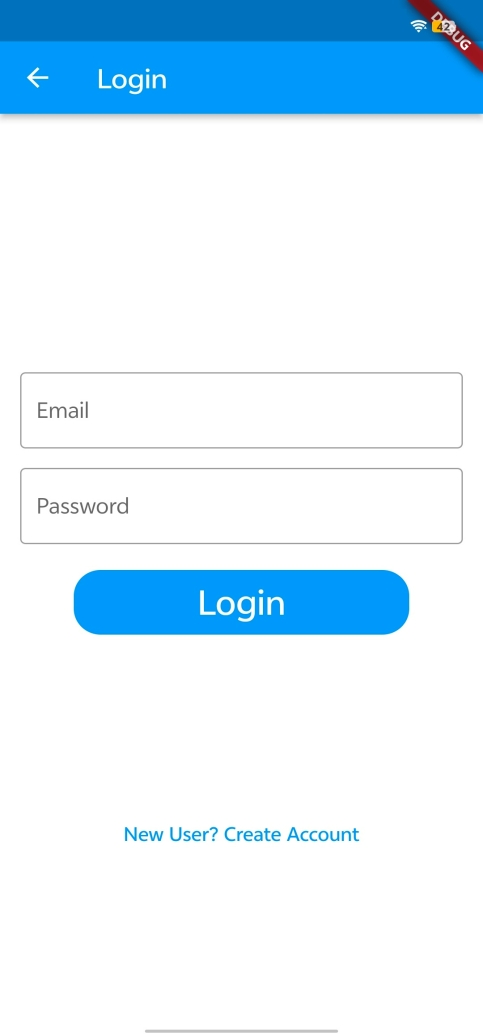
\includegraphics[scale=0.4]{pic/moblie/login.jpg} &   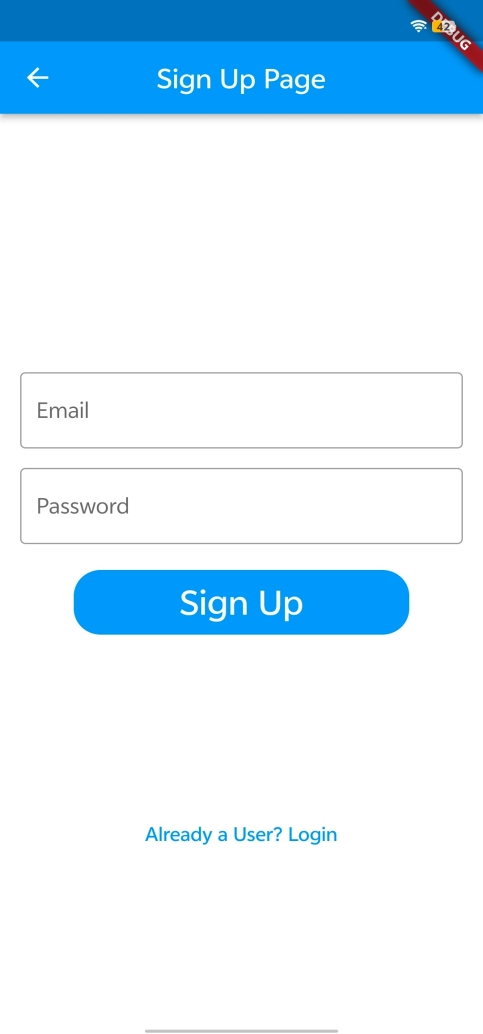
\includegraphics[scale=0.4]{pic/moblie/signup.jpg} \\
             Login &  Signup \\[6pt]
          
            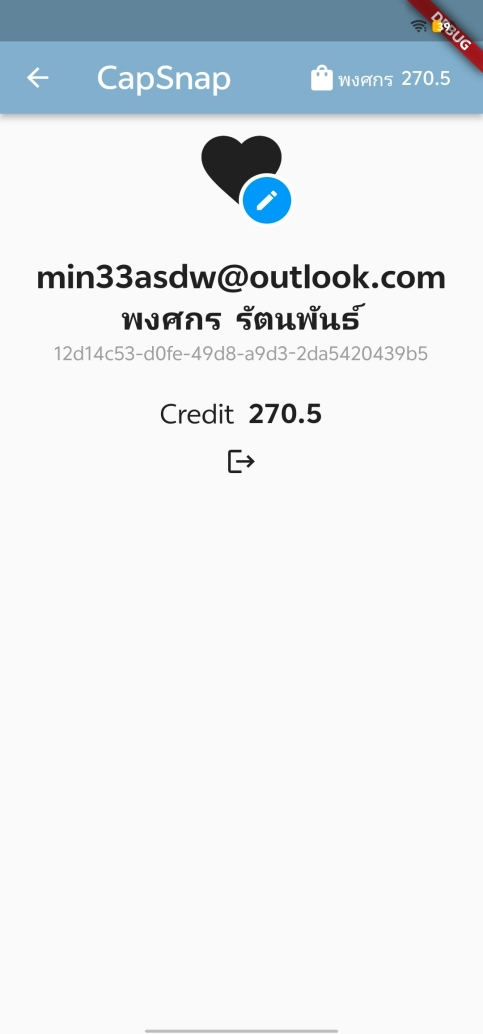
\includegraphics[scale=0.4]{pic/moblie/profile.jpg} &   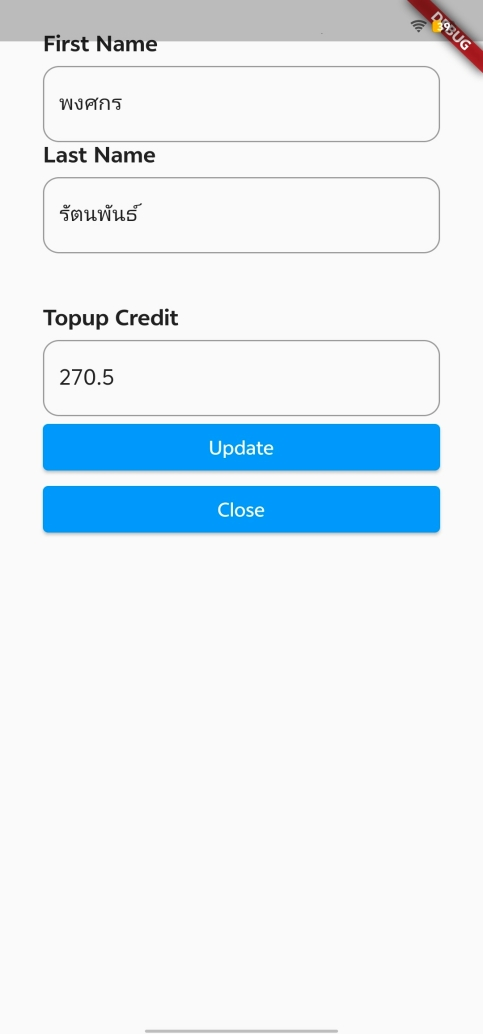
\includegraphics[scale=0.4]{pic/moblie/edit.jpg} \\
             Profile &  Edit profile \\[6pt]
            \end{tabular}
        \end{center}
    \end{figure}

    \begin{figure}
        \begin{center}
            \begin{tabular}{c@{\hspace{3cm}}c}
            
            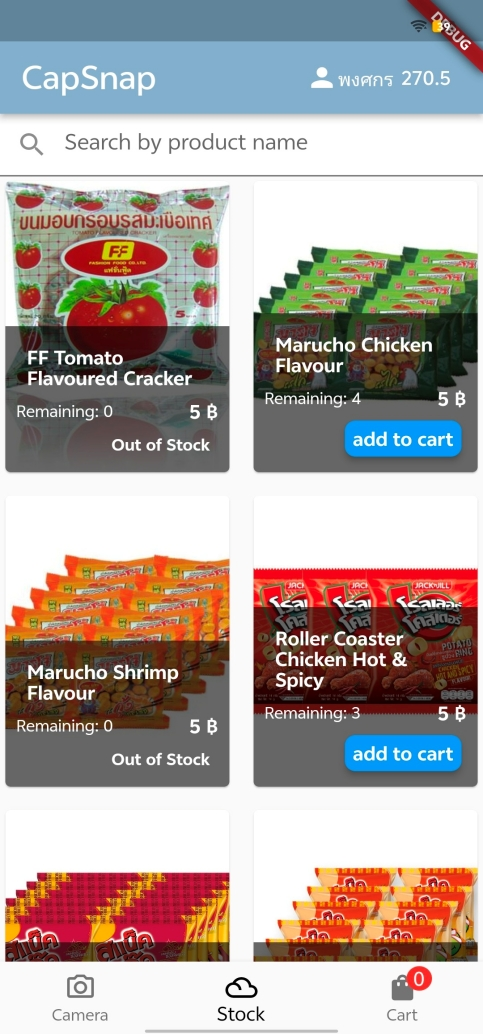
\includegraphics[scale=0.4]{pic/moblie/stock.jpg} &   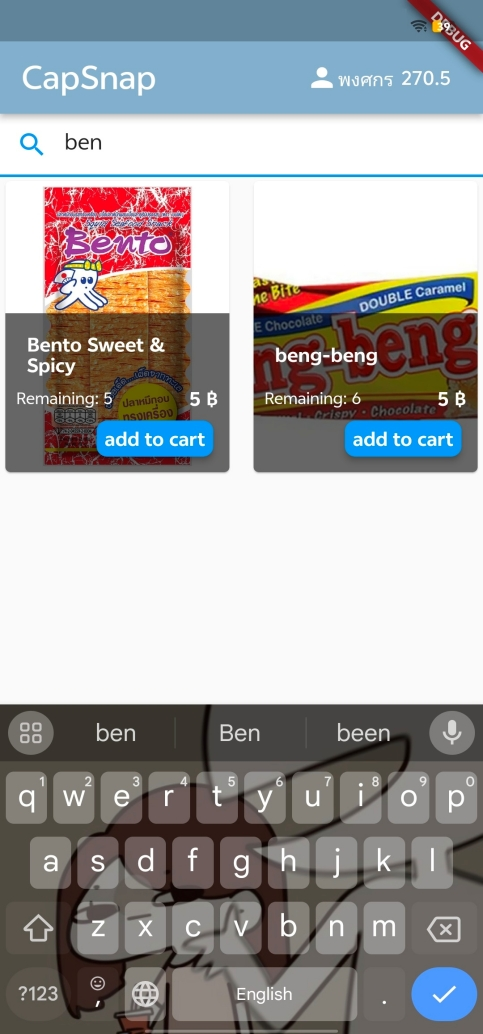
\includegraphics[scale=0.4]{pic/moblie/search_products.jpg} \\
             Stock & Search products \\[6pt]
          
            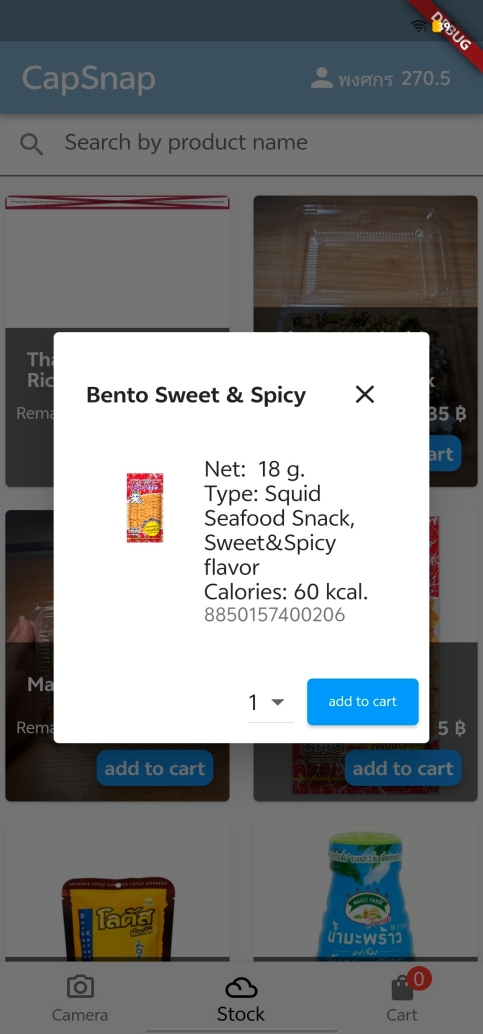
\includegraphics[scale=0.4]{pic/moblie/stock_detail.jpg} &   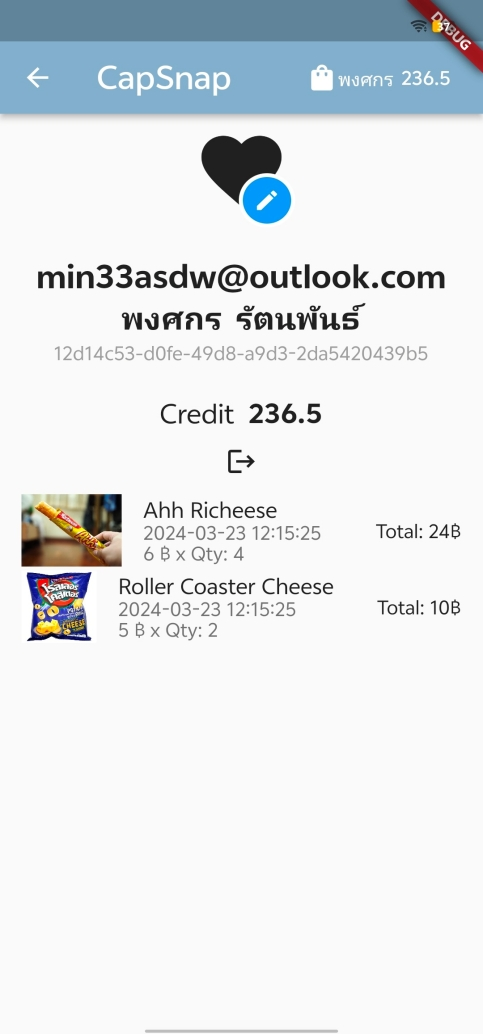
\includegraphics[scale=0.4]{pic/moblie/history.jpg} \\
            Product detail &  Purchase history \\[6pt]
            \end{tabular}
        \end{center}
    \end{figure}

    \begin{figure}
        \begin{center}
            \begin{tabular}{c@{\hspace{3cm}}c}
            
            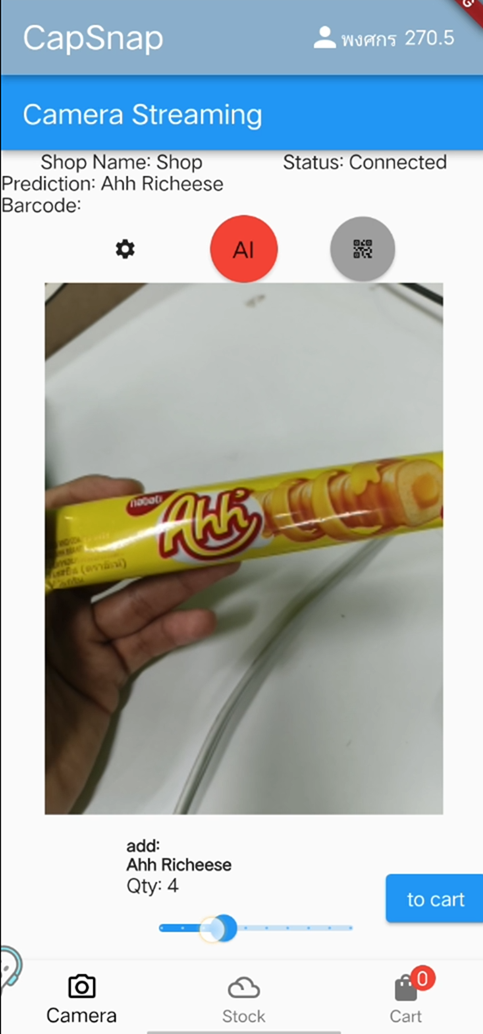
\includegraphics[scale=0.4]{pic/moblie/camera_ai.png} &   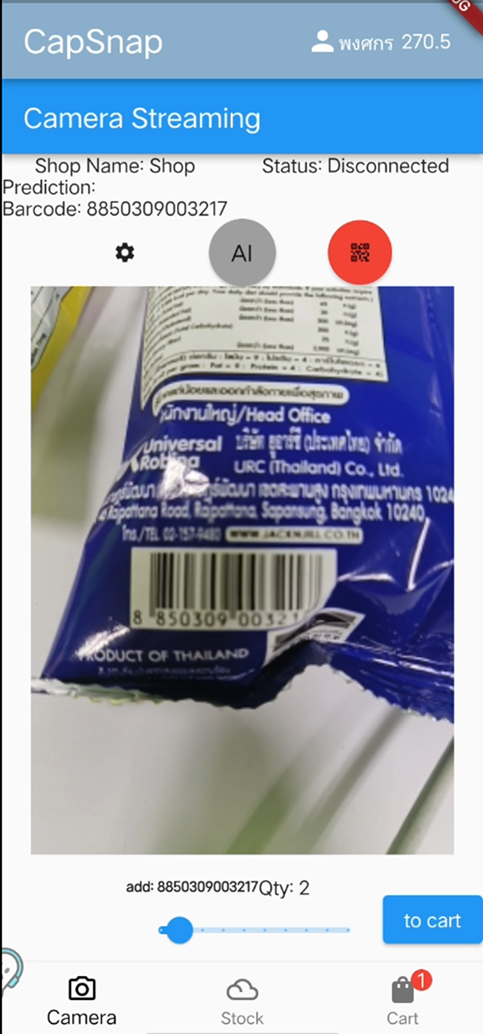
\includegraphics[scale=0.4]{pic/moblie/camera_barcode.png} \\
            Camera streaming  & Camera barcode \\[6pt]
          
            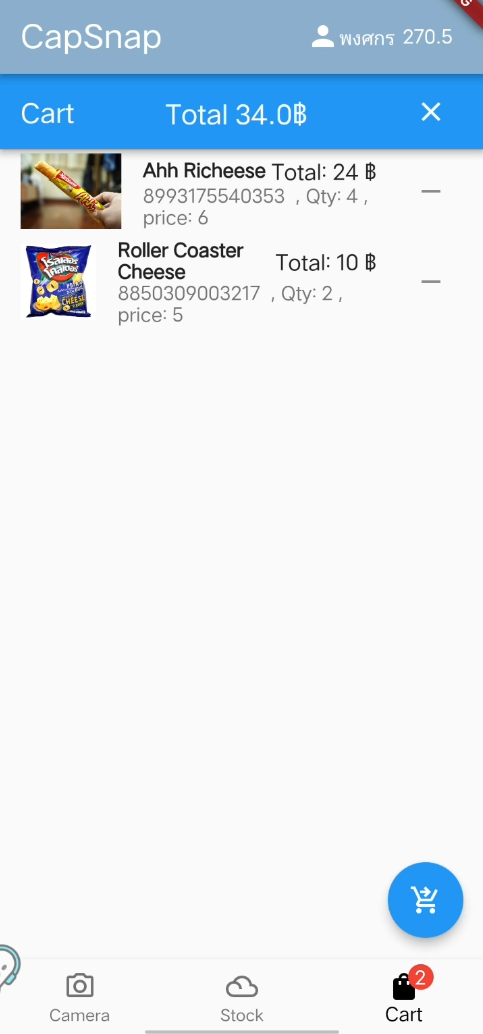
\includegraphics[scale=0.4]{pic/moblie/cart.png} &   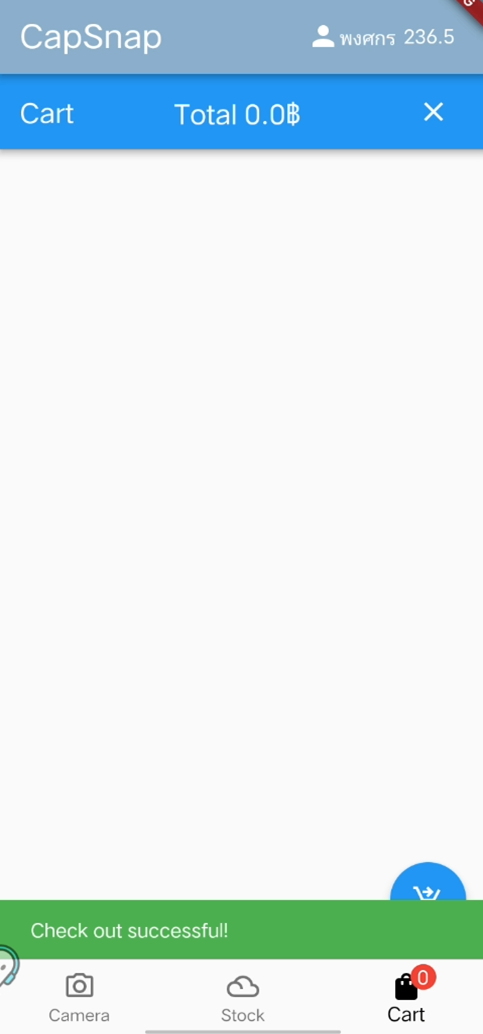
\includegraphics[scale=0.4]{pic/moblie/checkout.png} \\
            Cart  &  Checkout \\[6pt]
            \end{tabular}
        \end{center}
    \end{figure}
    % \begin{figure}[h]
    %     \begin{center}
   
    %         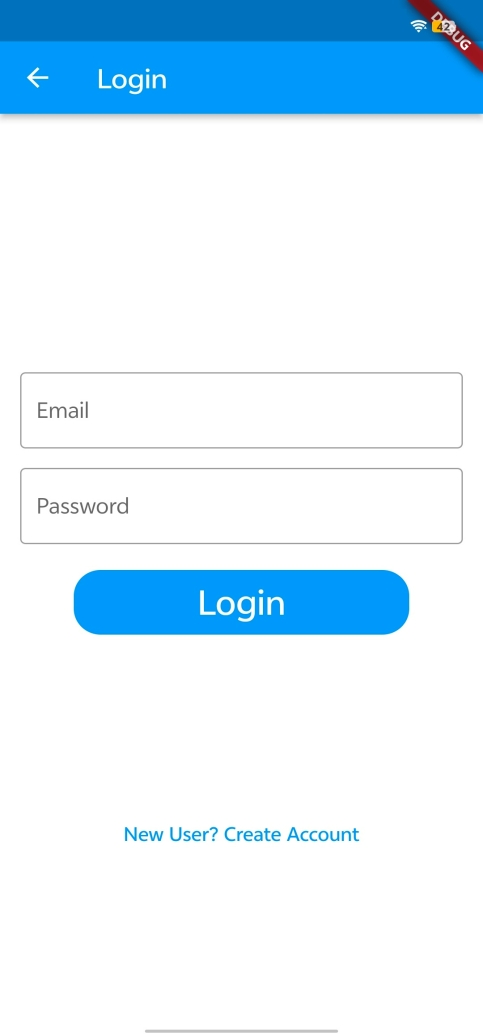
\includegraphics[scale=0.1]{pic/moblie/login.jpg}
    %     \end{center}
    
    %     \caption[App Login]{App Login}
    % \label{fig:App Login}
    % \end{figure} 

    % \begin{figure}[h]
    %     \begin{center}
   
    %         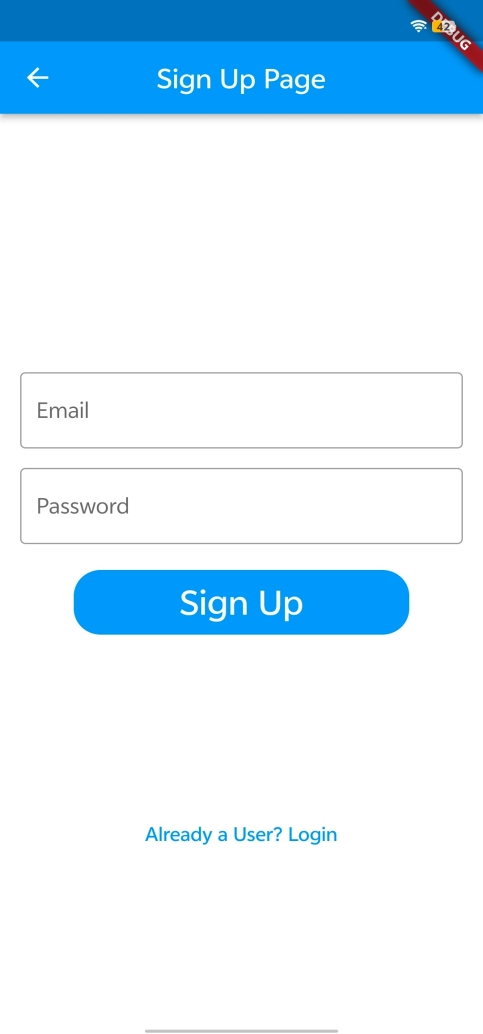
\includegraphics[scale=0.1]{pic/moblie/signup.jpg}
    %     \end{center}
    
    %     \caption[App signup]{App signup}
    % \label{fig:App signup}
    % \end{figure} 

    % \begin{figure}[h]
    %     \begin{center}
   
    %         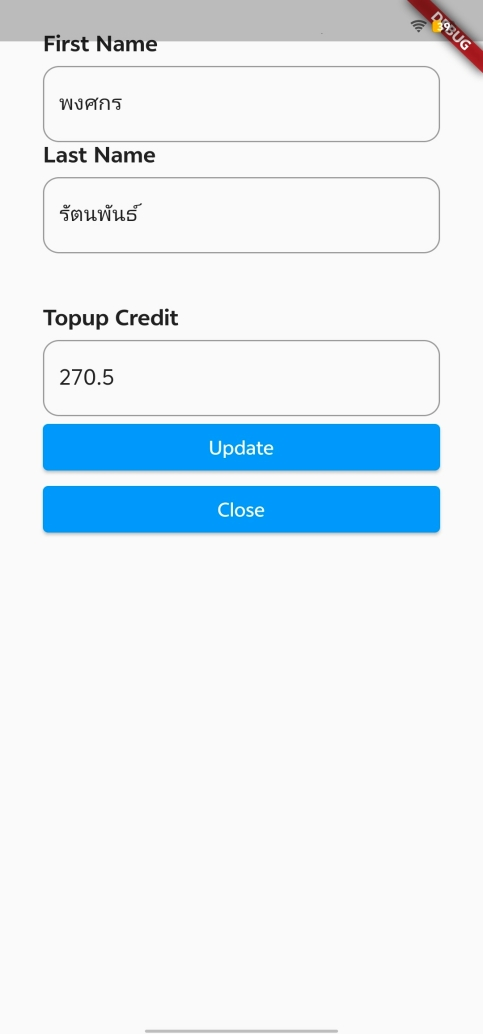
\includegraphics[scale=0.1]{pic/moblie/edit.jpg}
    %     \end{center}
    
    %     \caption[App edit]{App edit}
    % \label{fig:App edit}
    % \end{figure} 


\newpage
\section{Web Dashboard UX/UI}
    % \begin{center}
{
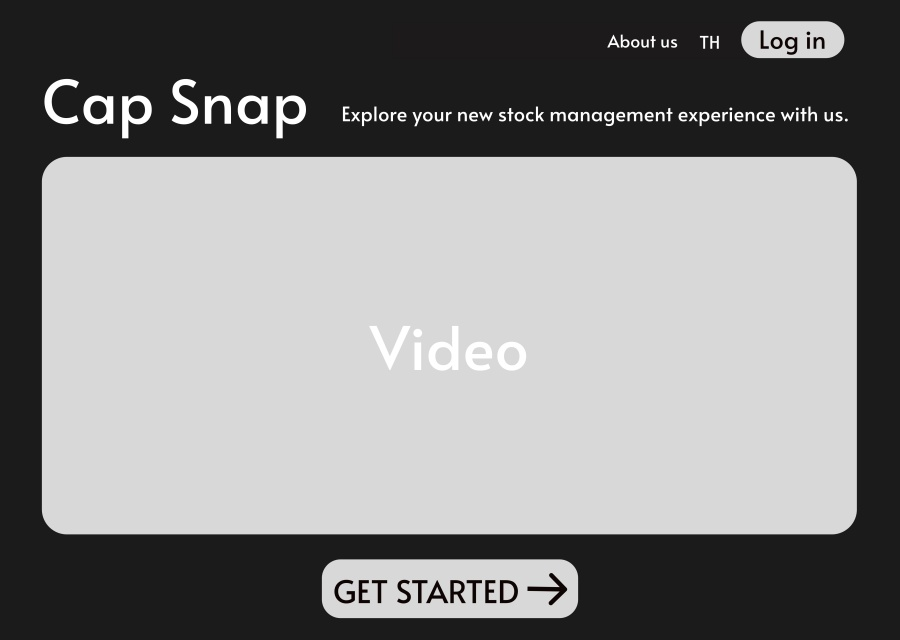
\includegraphics[scale=0.9]{pic/ui/1.jpg}
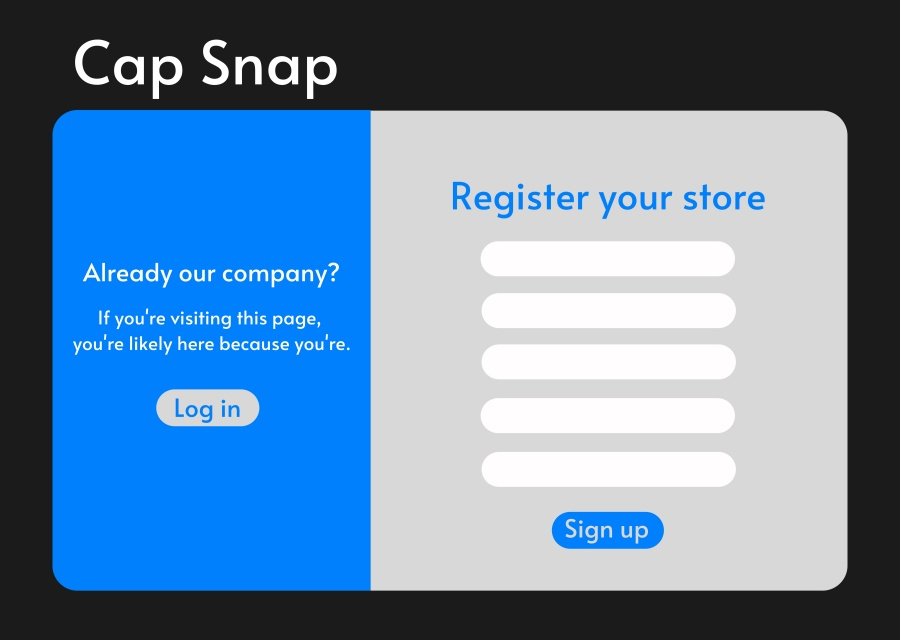
\includegraphics[scale=0.9]{pic/ui/2.jpg}
}\\
{
 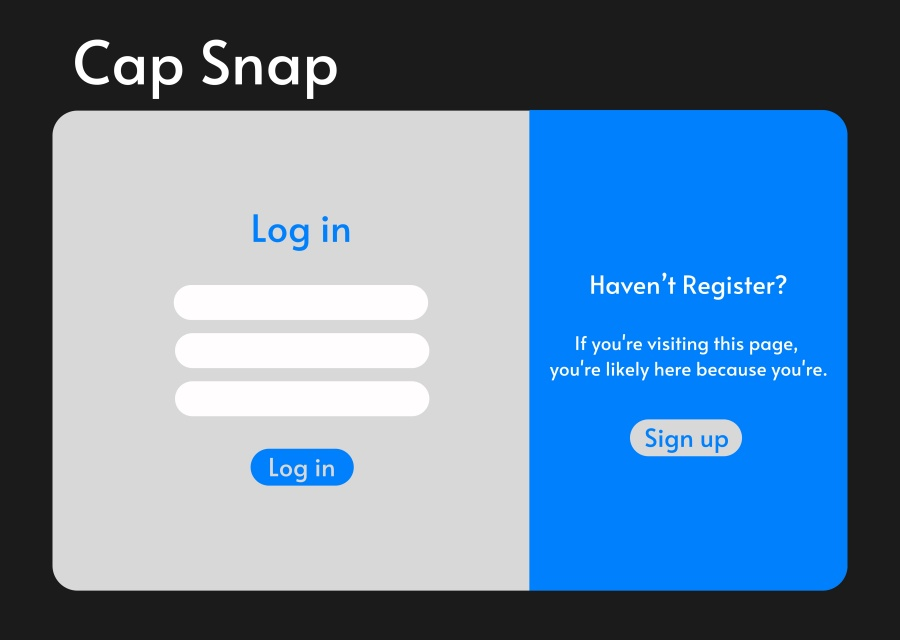
\includegraphics[scale=0.9]{pic/ui/3.jpg}
 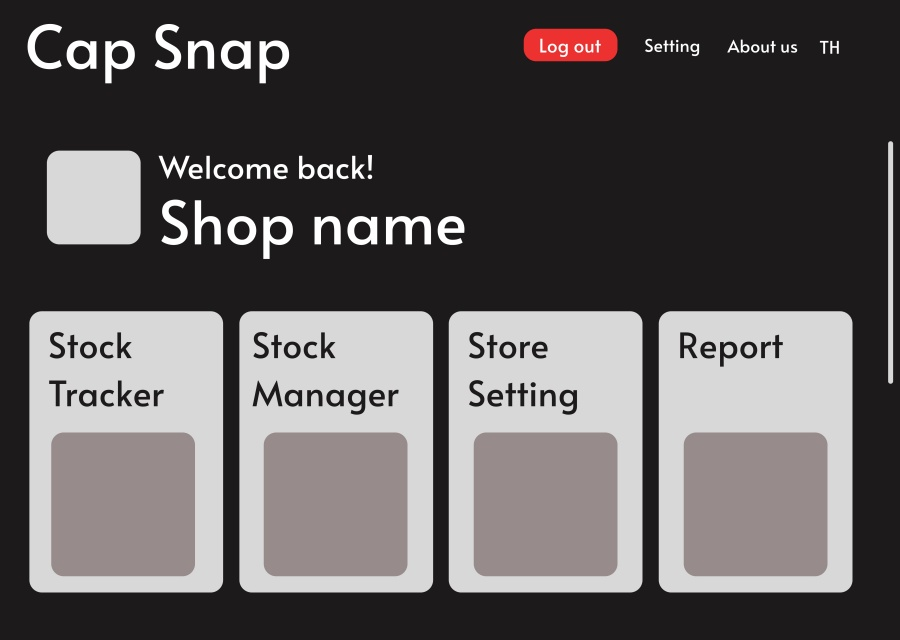
\includegraphics[scale=0.9]{pic/ui/4.jpg}
}\\
{
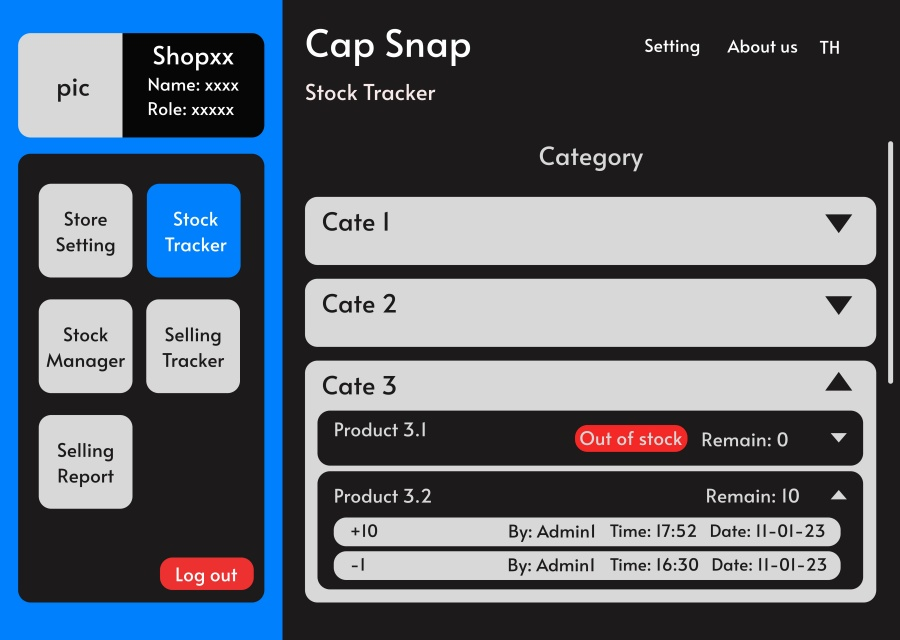
\includegraphics[scale=0.9]{pic/ui/5.jpg}
% 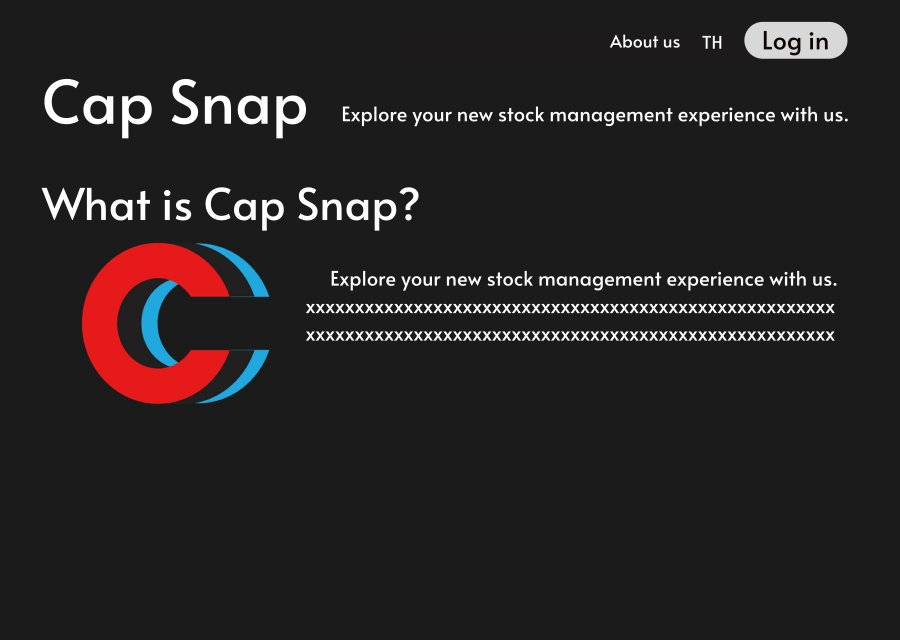
\includegraphics[scale=0.9]{pic/ui/6.jpg}
}\\
{
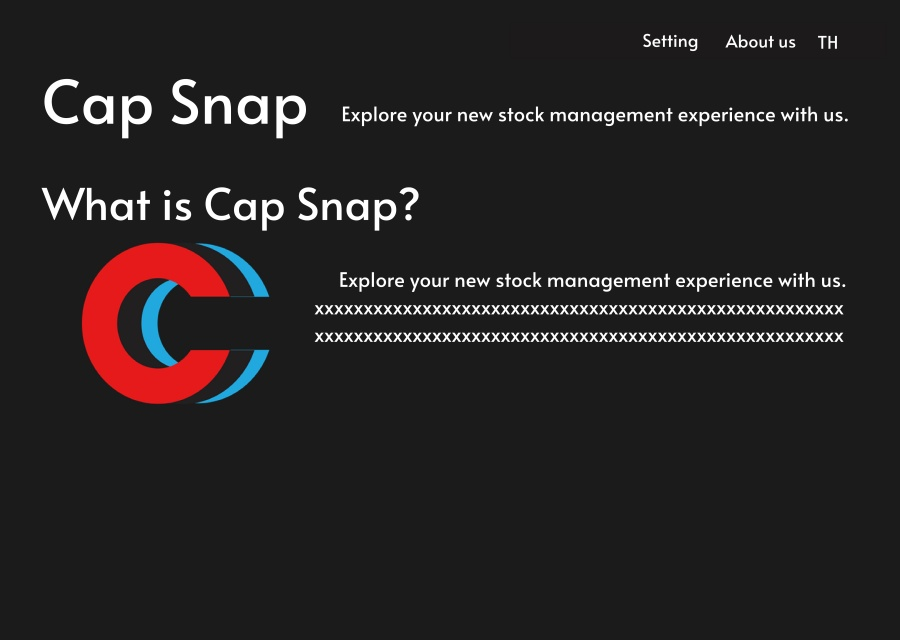
\includegraphics[scale=0.9]{pic/ui/7.jpg}
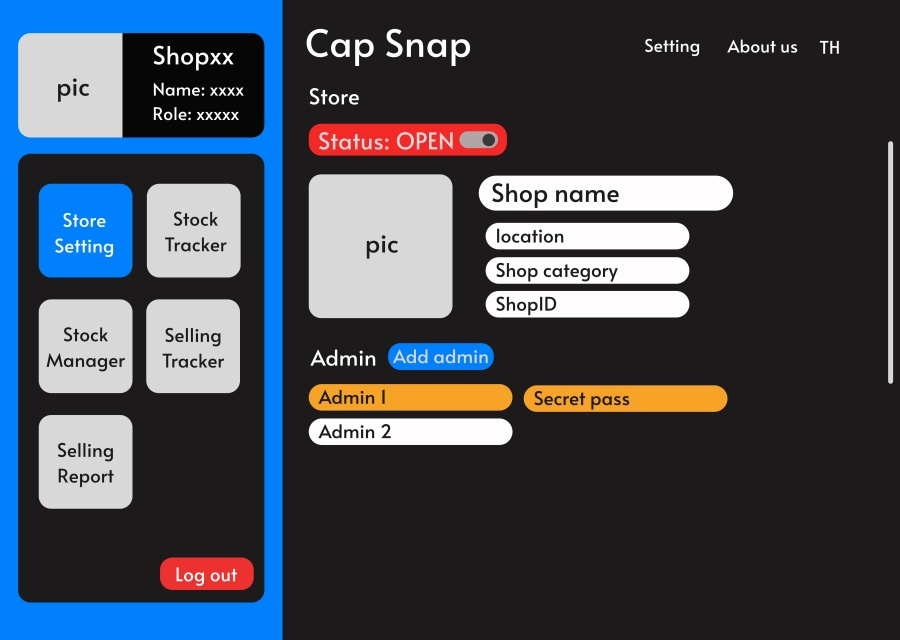
\includegraphics[scale=0.9]{pic/ui/8.jpg}
}\\
{
 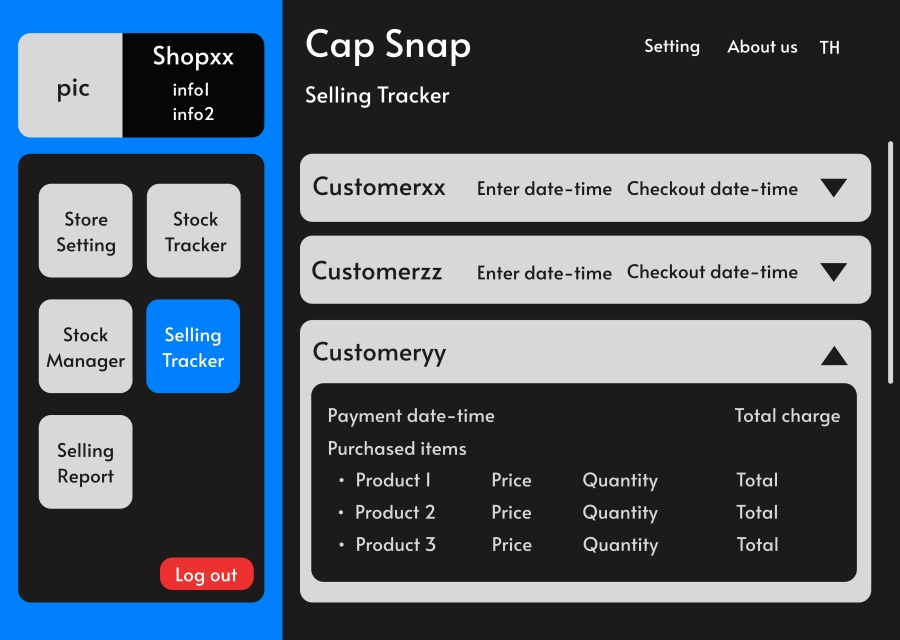
\includegraphics[scale=0.9]{pic/ui/9.jpg}
 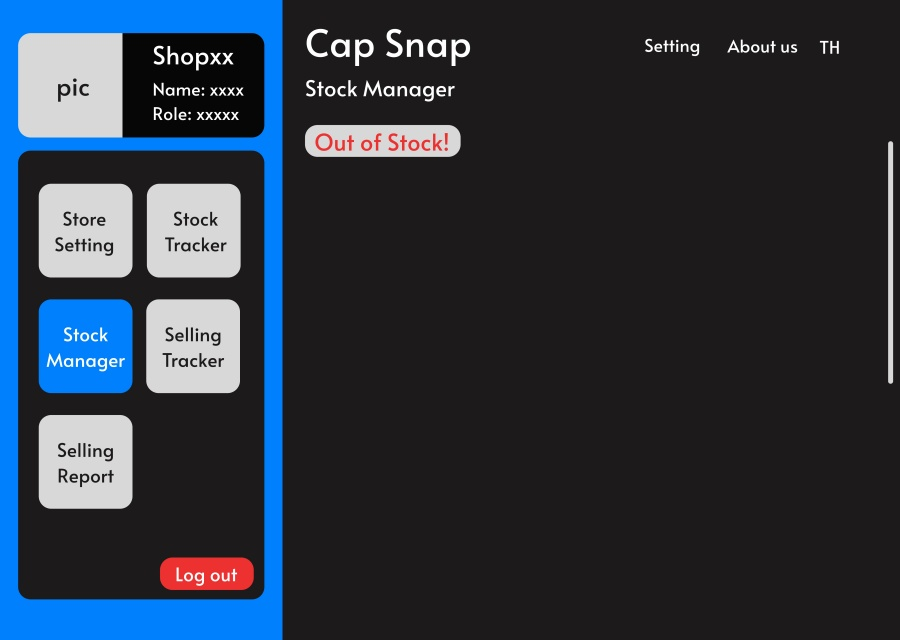
\includegraphics[scale=0.9]{pic/ui/10.jpg}
}\\
{
 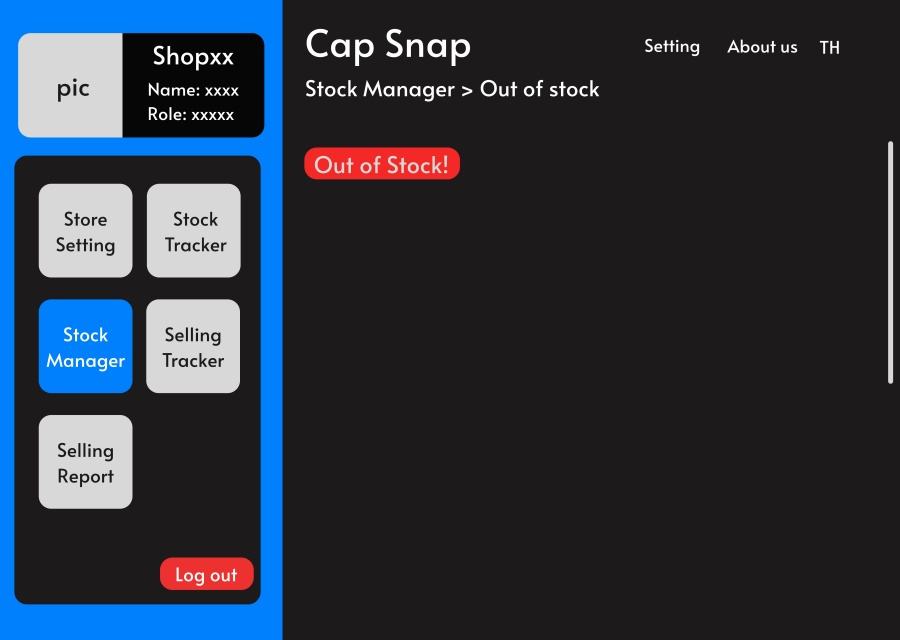
\includegraphics[scale=0.9]{pic/ui/11.jpg}
 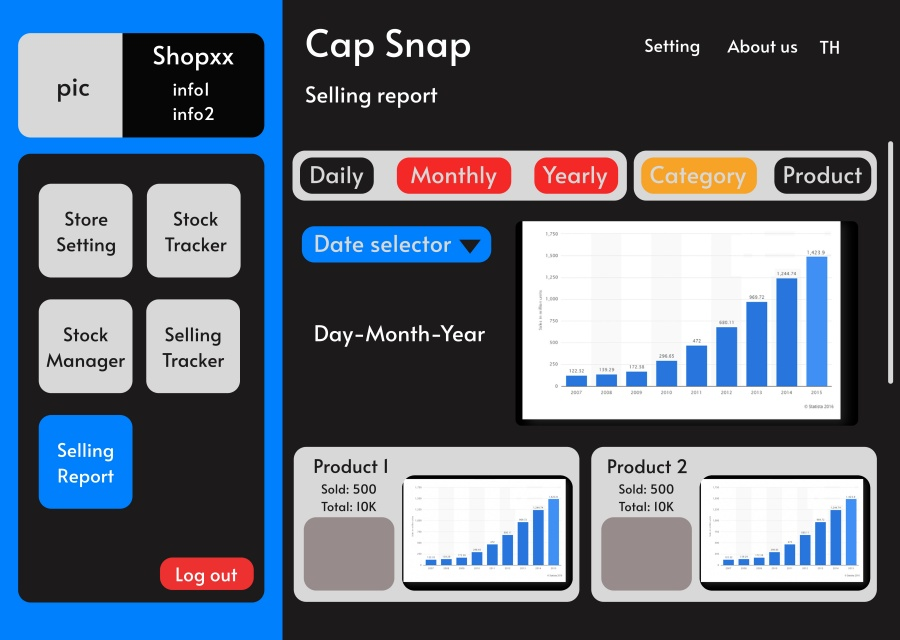
\includegraphics[scale=0.9]{pic/ui/12.jpg}
}


ในส่วนของการออกแบบส่วนสื่อประสานกับผู้ใช้ (GUI) ของ Website Dashboard นั้น ได้กำหนดให้มีหน้าการใช้งานหลักทั้งหมด 11 หน้า ได้แก่
\begin{enumerate}
    \item Get started page: หน้าการเข้าสู่ระบบ หรือลงทะเบียนเข้าใช้งาน
    \item Login page: หน้าการเข้าสู่ระบบ
    \item Register page: หน้าการลงทะเบียนเข้าใช้งาน
    \item Home page:  หน้าแสดงเมนูของฟังก์ชันต่าง ๆ
    \item Store setting page: หน้าการตั้งค่าข้อมูลร้านค้า
    \item Stock tracker page: หน้าการติดตามคลังสินค้า
    \item Stock manager page: หน้าการจัดการคลังสินค้า
    \item Stock manager page > Out of stock page: หน้าการจัดการสินค้าที่ไม่เหลือในคลัง
    \item Selling tracker page: หน้าการติดตามยอดขายตามลำดับคำสั่งซื้อ
    \item Selling report page: หน้าการแสดงผลข้อมูลยอดขายตามรายวัน รายเดือน และรายปี โดยสามารถดูตามหมวดหมู่ของสินค้า หรือแยกตามสินค้าหนึ่ง ๆได้
    \item About us page: หน้าแสดงรายละเอียดของผลิตภัณฑ์ของเรา
\end{enumerate}
 
 
% 1.	Get started page: หน้าการเข้าสู่ระบบ หรือลงทะเบียนเข้าใช้งาน
% 2.	Login page: หน้าการเข้าสู่ระบบ
% 3.	Register page: หน้าการลงทะเบียนเข้าใช้งาน
% 4.	Home page:  หน้าแสดงเมนูของฟังก์ชันต่าง ๆ
% 5.	Store setting page: หน้าการตั้งค่าข้อมูลร้านค้า
% 6.	Stock tracker page: หน้าการติดตามคลังสินค้า
% 7.	Stock manager page: หน้าการจัดการคลังสินค้า
% 8.	Stock manager page > Out of stock page: หน้าการจัดการสินค้าที่ไม่เหลือในคลัง
% 9.	Selling tracker page: หน้าการติดตามยอดขายตามลำดับคำสั่งซื้อ
% 10.	Selling report page: หน้าการแสดงผลข้อมูลยอดขายตามรายวัน รายเดือน และรายปี โดยสามารถดูตามหมวดหมู่ของสินค้า หรือแยกตามสินค้าหนึ่ง ๆได้
% 11.	About us page: หน้าแสดงรายละเอียดของผลิตภัณฑ์ของเรา

    
    % \end{center}

